\documentclass{article}
  \usepackage{amsmath}
  \usepackage{amssymb}
  \usepackage{graphicx}
  \usepackage{float}
\topmargin=-1.2cm \oddsidemargin=0.1cm \evensidemargin=0.1cm
\textwidth=16 true cm \textheight=23 true cm

\font\euler=EUSM10 \font\eulers=EUSM7

\begin{document}
\title{ECON 3610B International Trade \\Assignment $4^{\text{st}}$}
\author{{\normalsize Leonard Sheng(SHENG,Hao), 1155035947, via \LaTeX}}
\date{\today}

\maketitle
\baselineskip 0.6cm

\begin{description}
    \item[{\bf I. The Cost and Benefit of a Tariff}]:\\
    Let's denote the price at Home as $P$; the price at Foreign as $P^*$.
    \begin{description}
      \item[1.]
      \begin{align}
        \text{MD}=D-S=80-40P
      \end{align}
      When there isn't any trade, we have:
      \begin{align}
        D-S&=\text{DM}=0\\
        \text{thus,   }P&= 2
      \end{align}
      \begin{center}
                 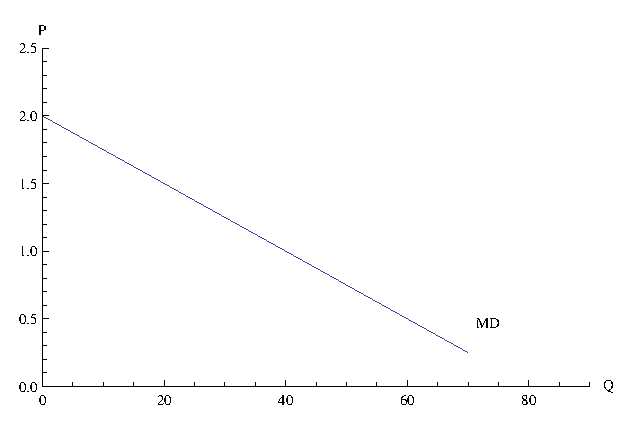
\includegraphics[angle=0, width=0.6\textwidth]{ECON3610BA4P1}
      \end{center}
    \item[2.]
      {\bf (a):}
      \begin{align}
        \text{ES}=S^*-D^*=-40+40P^*
      \end{align}
      When there isn't any trade, we have:
      \begin{align}
       S^*-D^*&=\text{ES}=0\\
        \text{thus,   }P&= 1
      \end{align}
      \begin{center}
                 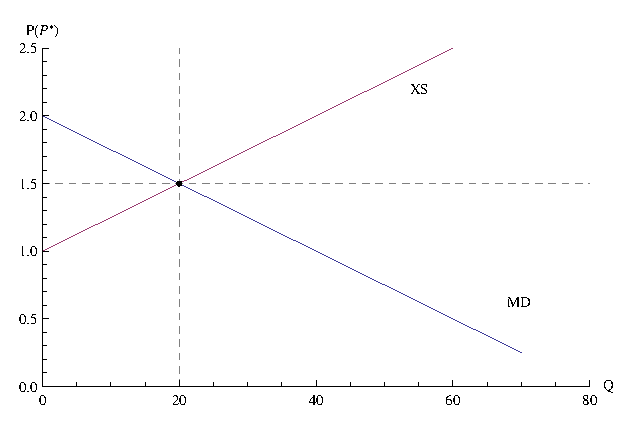
\includegraphics[angle=0, width=0.6\textwidth]{ECON3610BA4P2}
      \end{center}
      {\bf (b):}
      Now the trade begin:
      \begin{align}
        \begin{cases}
         80-40P&=\text{DM}=\text{ES}=-40+40P^* \\
         P&=P^*
        \end{cases}
      \end{align}
      Solve it, we have:
      \begin{align}
         P=P^*=1.5\\
         \text{XS}=\text{MD}=20
      \end{align}
    \item[3.]
      {\bf (a):}Now, we have:
      \begin{align}
        \begin{cases}
            80-40P&=\text{DM}=\text{ES}=-40+40P^* \\
            P&=P^*+0.5
        \end{cases}
      \end{align}
      Solve it, we get: \begin{align}
        P&=1.75, P^*=1.25\\
        D&=100-20P=65\\
        S&=20+20P=55\\
        D^*&=80-20P^*=55\\
        S^*&=40+20P=65\\
        \text{XS}&=\text{MD}=10
        \end{align}
        The effects are graphed in the next page.
        \begin{figure}[H]\centering
        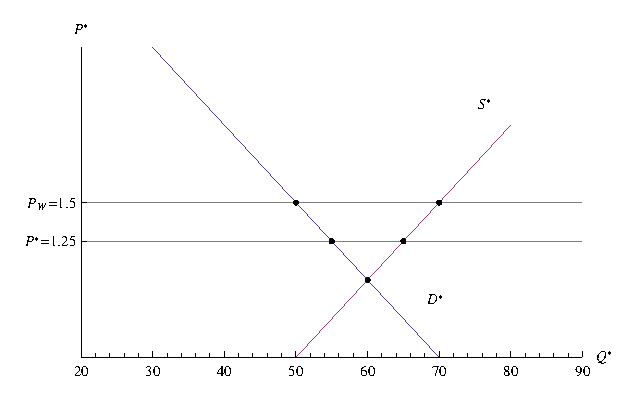
\includegraphics[angle=90,width=.3\textwidth]{ECON3610BA4P5}\\
        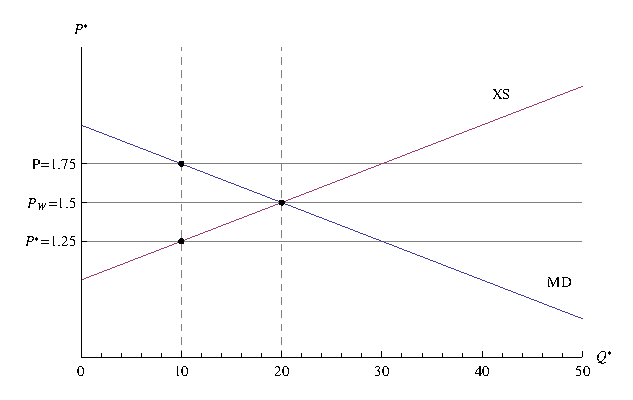
\includegraphics[angle=90,width=.3\textwidth]{ECON3610BA4P4}\\
        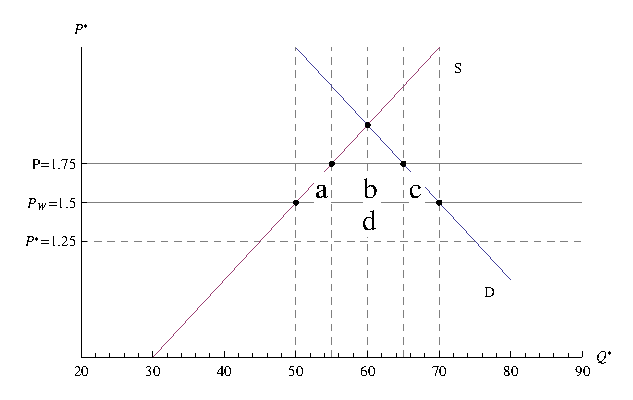
\includegraphics[angle=90,width=.3\textwidth]{ECON3610BA4P3}\\
        \end{figure}
      {\bf (b):}
      \begin{align}
        \text{Change of Home import-competing producers' welfare}&=\frac{(55+50)}{2}*(1.75-1.5)=13.125\\
        \text{Change of Home consumers' welfare}&=-\frac{(70+65)}{2}*(1.75-1.5)=-16.875\\
        \text{Gains of the Home government}&=0.5*(65-55)=5
      \end{align}
      {\bf (c):}
      \begin{align}\notag
        \text{Efficiency loss}&=-(a+c)=(\frac{(55+50)}{2}-\frac{(70+65)}{2})*(1.75-1.5)+0.5*5\\  &=-1.25\\
        \text{The terms of trade gain}&=d=0.5*(60-55)=2.5\\
        \text{Total effect on welfare}&=-(a+c)+d=1.25
      \end{align}
      \item[4.]
        \begin{align}
        \text{DM}&=D-S=80-40P\\
        \text{ES}&=S^*-D^*=-400+400P^*
        \end{align}
         When there is no tariff:
        \begin{align}
        \begin{cases} \text{DM}=80-40P=\text{ES}=-400+400P^* \\
                P=P^*
        \end{cases}
        \end{align}
        gives us the equilibrium:
        \begin{align}
          P&=P^*=\frac{12}{11}\doteq 1.09\\
          \text{DM}&=\text{ES}=\frac{400}{11}\doteq 36.4
        \end{align}
        As the tariff is levied:
        \begin{align}
          \begin{cases}
            \text{DM}=80-40P=\text{ES}=-400+400P^* \\
             P=P^*+0.5\end{cases}
        \end{align}
        gives us the equilibrium:
        \begin{align}
          P^*&=\frac{23}{22}\doteq 1.045\\
          P&=\frac{34}{22}\doteq 1.545\\
          \text{DM}&=\text{ES}=\frac{200}{11}\doteq 18.2
        \end{align}
        \begin{center}
                 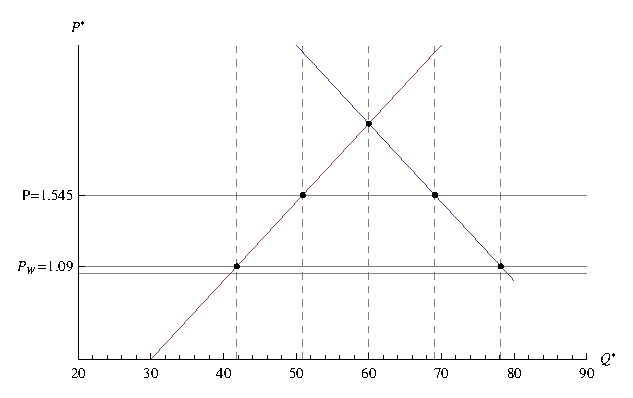
\includegraphics[angle=0, width=0.6\textwidth]{ECON3610BA4P6}
        \end{center}
        Now,
        \begin{align}\notag
        \text{Efficiency loss}&=(\frac{\frac{460}{11}+\frac{560}{11}}{2}-\frac{\frac{860}{11}+\frac{760}{11}}{2})*\left(\frac{34}{22}-\frac{12}{11}\right)+\left(\frac{34}{22}-\frac{12}{11}\right)*\left(\frac{760}{11}-\frac{560}{11}\right)\\  &\doteq -4.13\\
        \text{The terms of trade gain}&=\left(\frac{12}{11}-\frac{23}{22}\right)*\left(\frac{760}{11}-\frac{560}{11}\right)\doteq 0.826\\
        \text{Total effect on welfare}&\doteq -3.3
      \end{align}
      As we can see, even though the Foreign has been a much larger country, Home can still have at least some gains from the terms of trade after a tariff is levied. By and large, however, the smaller the country, the less it will gain from terms of trade(once begins a tariff). And we can see from this example, the efficiency loss may outweigh the gains, which makes tariff policy undesirable for the home as a small country.
\end{description}
    \item[{\bf II. Short Question on Trade Policy}]:\\
        The result of tariff is ambiguous. Large countries may gains from the tariff. However, this may not be true in the U.S, since it's a food export rather than import country.\\
        The main reason is that the cost of tariff, quota or subsidize are distributed among lots of people, probably all the consumers with in a nation; however, the benefit are concentrated in a few farmers. We can use the model of {\it collective action model} in Chap.10 to explain this phenomenon in democratic countries: farmers are small, well-organized group that is well aware of the size of benefits each member will receive from such policy, while consumers are a huge population that does not even perceive itself as an interest group. As a result, policy towards farmers may get more votes and moneys even though it may hurt far more voters.

    \item[{\bf III. Short Questions on Trade Policy}]:\\
    {\bf (1):}It's a valid argument for a tariff. Since the U.S. is a large oil-importing country, once it raise a tariff, the price in oil-exporting country will go down considerably. This may improve the terms of trade in the U.S. If the gains from the terms of trade is larger than the efficiency loss from the tariff, the whole nation will get better.\\
    {\bf (2):}It's not a valid argument for tariffs or export subsidies. Even though the exports of off-season fruit from Chile makes 80 percent of the U.S. supply, we don't know the share of Chile's export towards the U.S. in its total export amount. Once a tariff is levied, lot of U.S. consumers get hurt, while we don't know if how much the exporting-price in Chile and the rest of the world will get down. Thus we are not sure the gains from the terms of trade will cover the efficiency loss.\\
    {\bf (3):}It's not a valid argument for tariffs or export subsidies. Generally speaking, the loss of welfare as a overall nation is inevitable for subsidies, unless a domestic market failure. This argument implicates that there is positive externality for export-subsidies in foods sector, since the producer in that sector is richer. However, this will happen in other sectors if there is a export subsidies. It's not a true externality here.\\
    {\bf (4):}It's not a valid argument for tariffs or export subsidies. It implicates that there is positive externality for protection in semiconductors sector, since this will benefit other sectors. For domestic market failure, a domestic policy is usually cheaper. And we should use direct policy in order to avoid the further externality. In this case, government can use production subsidy.\\
    {\bf (5):}It's not a valid argument for tariffs or export subsidies. Almost all the consumers, including these unemployed workers are getting better from the decrease of timber price. If the policy's aim is to solve the unemployment problem, it's better to subsidize timber workers, helping them to transfer to other sectors.
    \item[{\bf IV. International Coordination}]:\\
    As is illustrated in Chap.10, in most cases (especially there are numerous countries and each country makes only a small part in total import and export amount), free trade is a better response even though the opponents in the game choose protection policy. Based on this, we can make a pay-off table like this:
    \begin{center}
      % Table generated by Excel2LaTeX from sheet 'Sheet1'
\begin{tabular}{rrcc}

           &            & \multicolumn{ 2}{c}{{\bf China}} \\

           &            & Free trade & Protection \\

\multicolumn{ 1}{c}{{\bf The.U.S.}} & Free trade &      20,20 &       5,15 \\

\multicolumn{ 1}{c}{{\bf }} & Protection &       15,5 &        0,0 \\

\end{tabular}

    \end{center}
    This game is no longer a Prisoner's dilemma.\\
    Since the choice $Protection$ is dominated by the choice $Free trade$, both China and the U.S. will choose free trade no matter what their opponent will do. The Nash equilibrium is that both countries pick up Free trade policy.
\end{description}
\end{document}
